\documentclass[slidestop, compress, mathserif]{beamer}
\usepackage[style=authoryear-comp, sorting=nyt, maxcitenames=2, backend=biber]{biblatex}
\renewbibmacro{in:}{}
\renewcommand\bibfont{\small}
\addbibresource{ref_01.bib}
\addbibresource{ref_02.bib}
\addbibresource{ref_03.bib}
\addbibresource{trappe.bib}

\usepackage{amsmath, amssymb, mathrsfs}
\usepackage{color, graphicx}

\usepackage{setspace, listings}
\usepackage{sidecap}

\usetheme{Madrid}
\usecolortheme{default}
\linespread{1.2}



\sidecaptionvpos{figure}{c}
\usepackage[textfont=small]{caption}
\setbeamertemplate{caption}[numbered]
\captionsetup{font=scriptsize, labelfont=scriptsize, labelformat=simple}

\setbeamertemplate{footline}
{
  \leavevmode%
  \hbox{%
  \begin{beamercolorbox}[wd=1.0\paperwidth,ht=2.25ex,dp=1ex]{author in head/foot}\usebeamerfont{author in head/foot}
    \hspace*{3ex}
    \inserttitle
    \hfill
    \insertshortauthor
    \hspace*{3ex}
  \end{beamercolorbox}%
}%
  \vskip0pt%
}


\title{Simulation in Equilibrium}
\author{Gun Woo Park}
% \institute{DICMaPI, University of Naples Federico II}
% \author{Gun Woo Park, Antonio Brasiello, and Giovanni Ianniruberto}
% \date{SUPOLEN PROJECT MEETING\\ 27 MAR 2015}


% it's for headline
% \setbeamertemplate{headline}{%
%   % \leavemode%
%   \hbox{%
%     % \begin{beamercolorbox}[wd=\paperwidth,ht=2.5ex,dp=1.125ex]{palette quaternary}%
%     \begin{beamercolorbox}[wd=\paperwidth,ht=2.5ex,dp=1.125ex]{section in head/foot}%
%       \insertsectionnavigationhorizontal{\paperwidth}{}{\hskip0pt plus1filll}
%     \end{beamercolorbox}%
%     }
% }

\begin{document}

\begin{frame}[plain]
\maketitle
\end{frame}


\begin{frame}
  \frametitle<presentation>{fNAS check}
  \begin{figure}
    \centering
    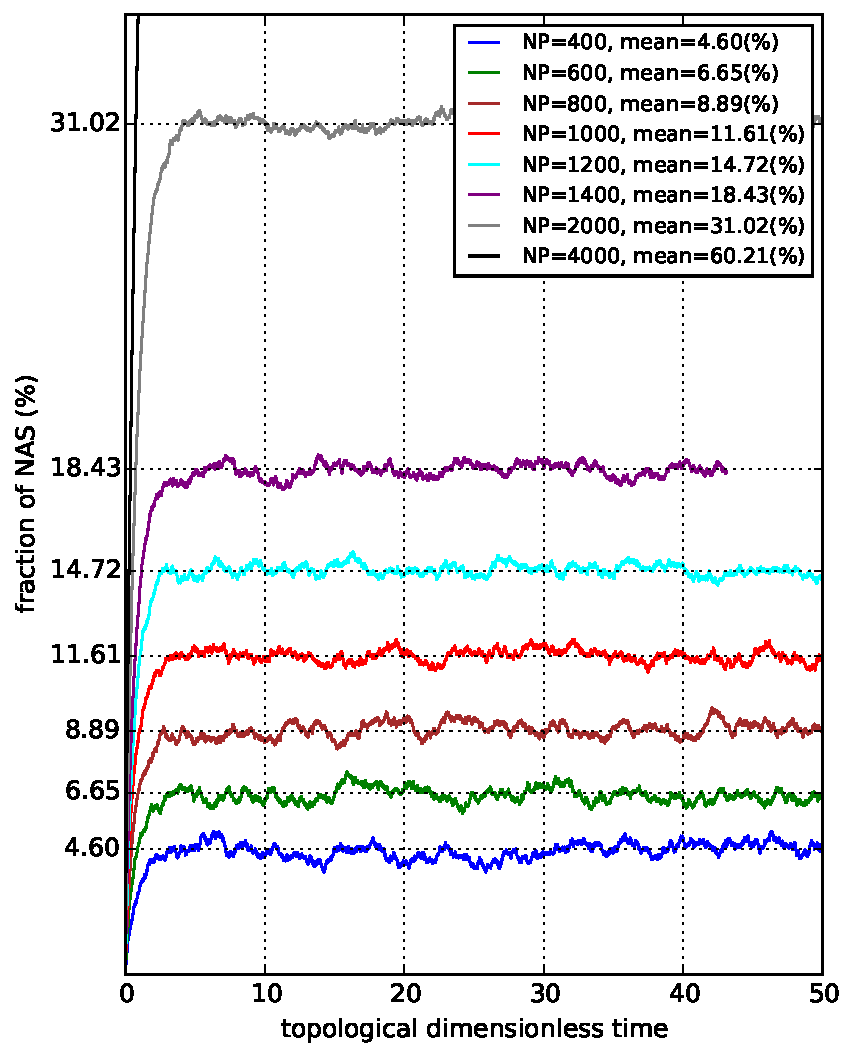
\includegraphics[width=0.45\textwidth]{../check_fNAS.pdf}
    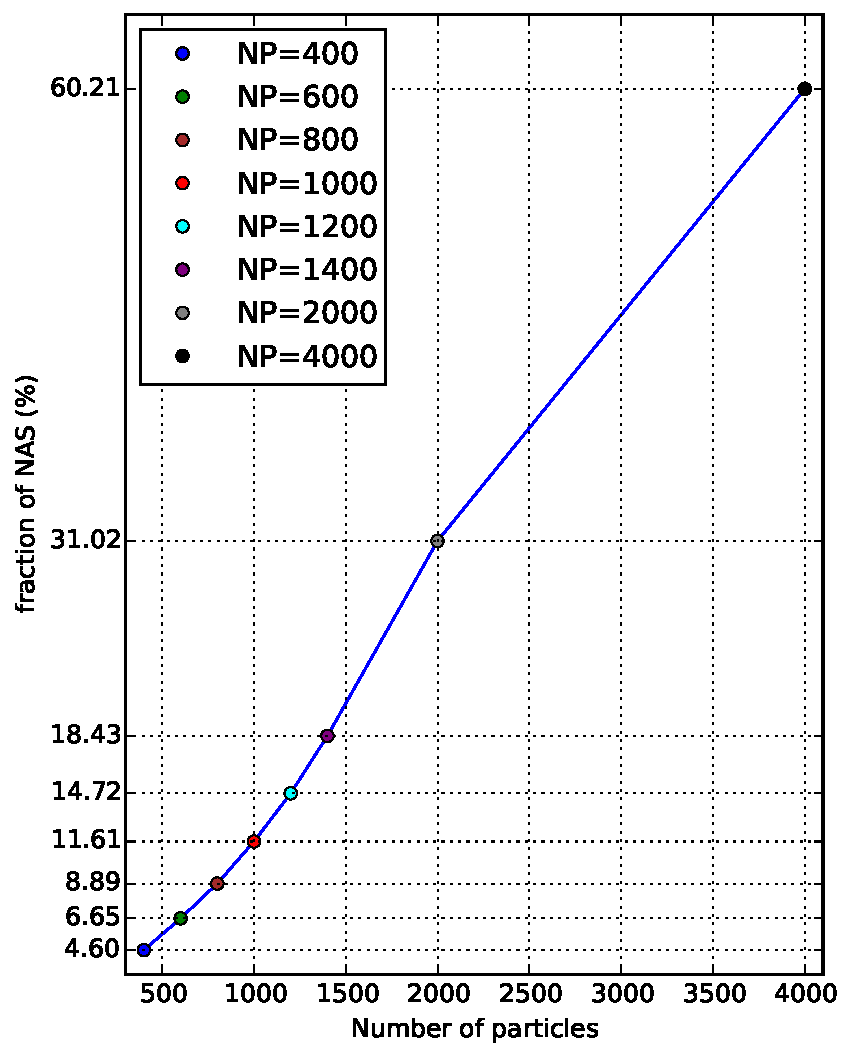
\includegraphics[width=0.45\textwidth]{../check_fNAS_NP.pdf}
  \end{figure}
\end{frame}

\begin{frame}
  \frametitle<presentation>{Shear Stress}
  \begin{figure}
    \centering
    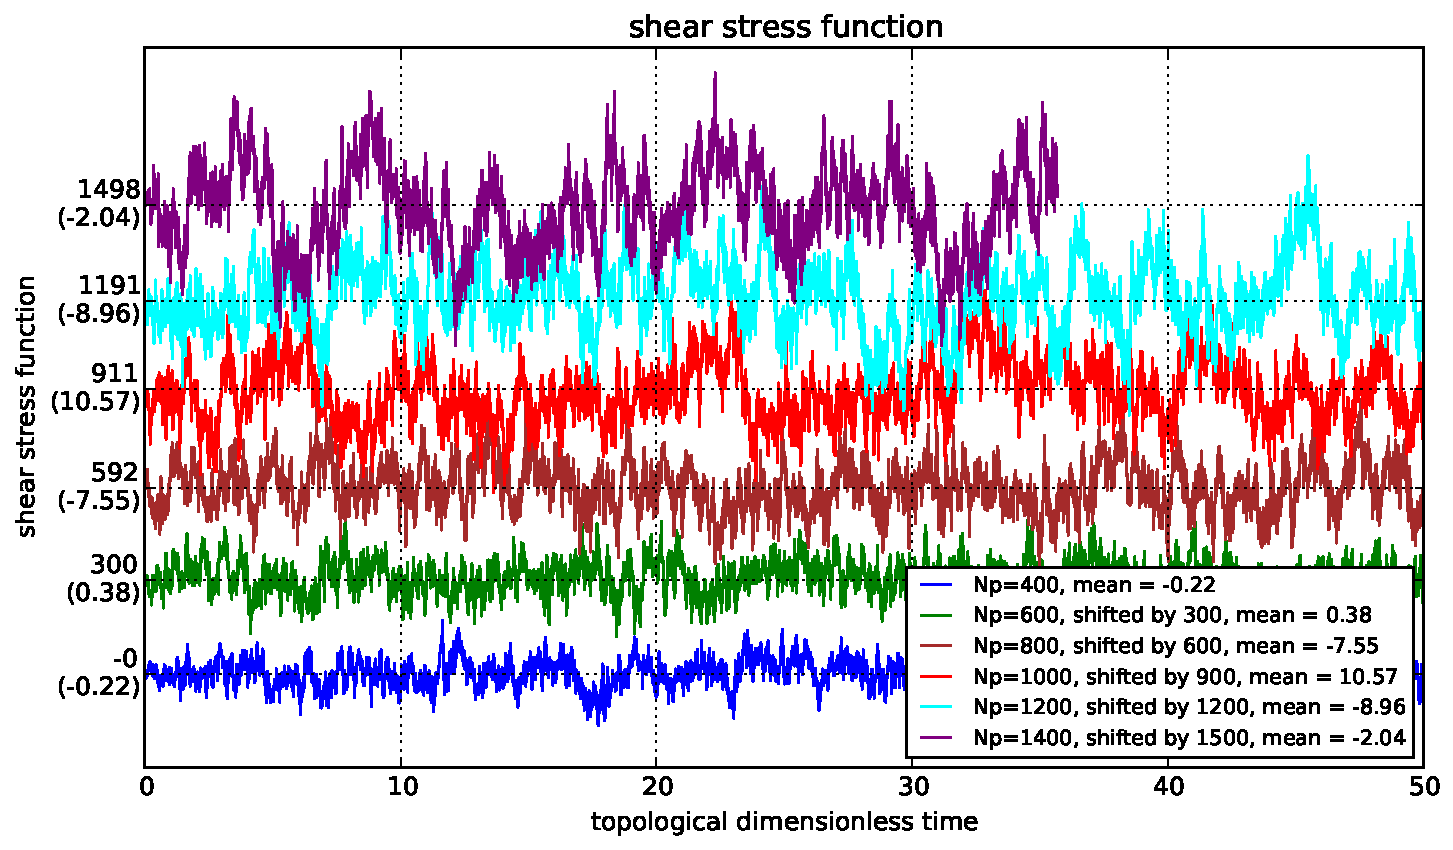
\includegraphics[width=\textwidth]{../shear_stress_function.pdf}
  \end{figure}
\end{frame}

\begin{frame}
  \frametitle<presentation>{Shear Stress, concentrated regime}
  \begin{figure}
    \centering
    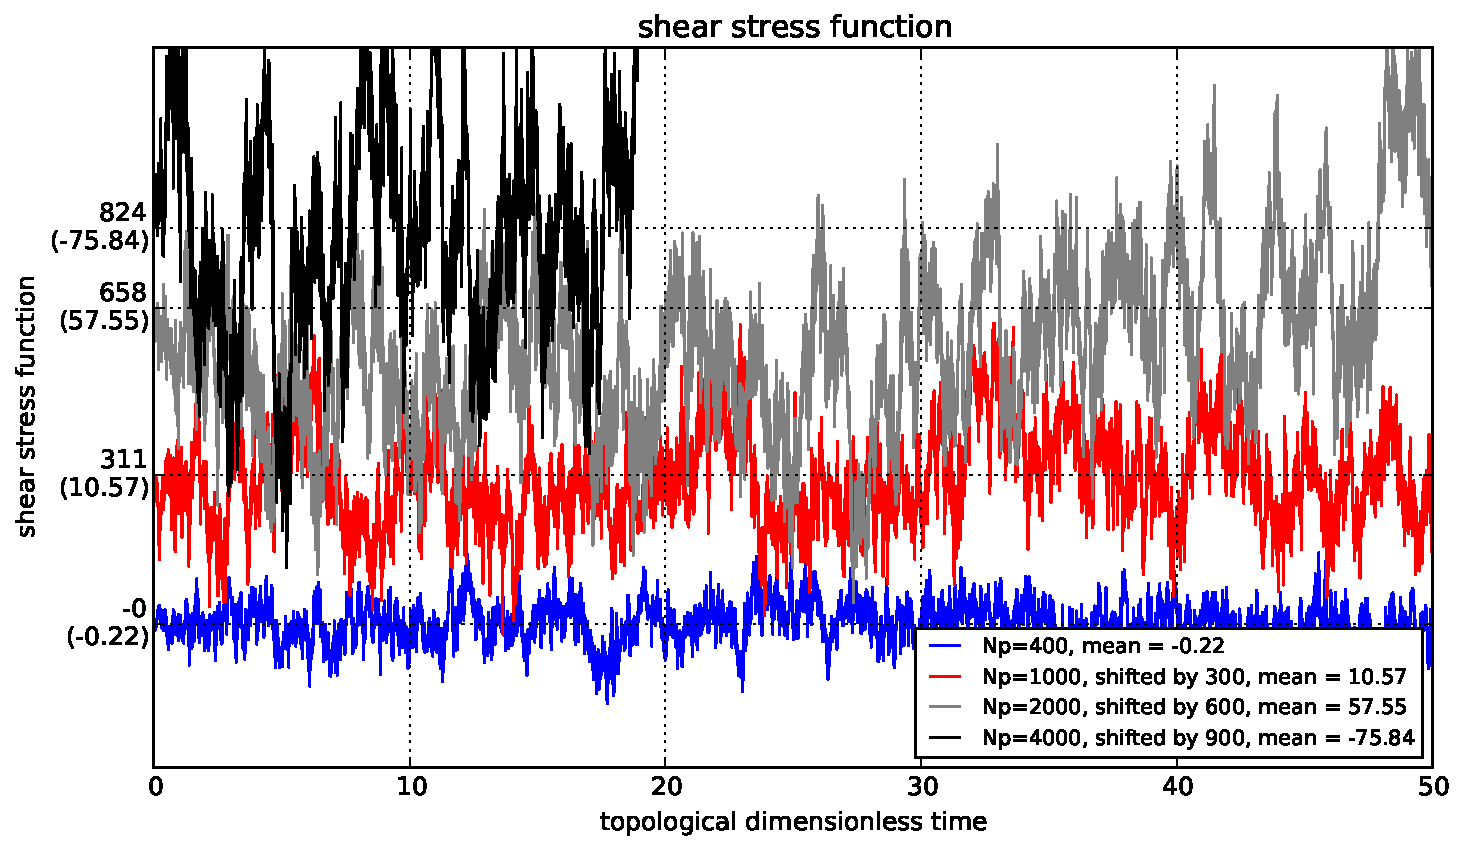
\includegraphics[width=\textwidth]{../shear_stress_function_over.pdf}
  \end{figure}
\end{frame}

\begin{frame}
  \frametitle<presentation>{ACF for Shear Stress, biased statistics}
  \begin{figure}
    \centering
    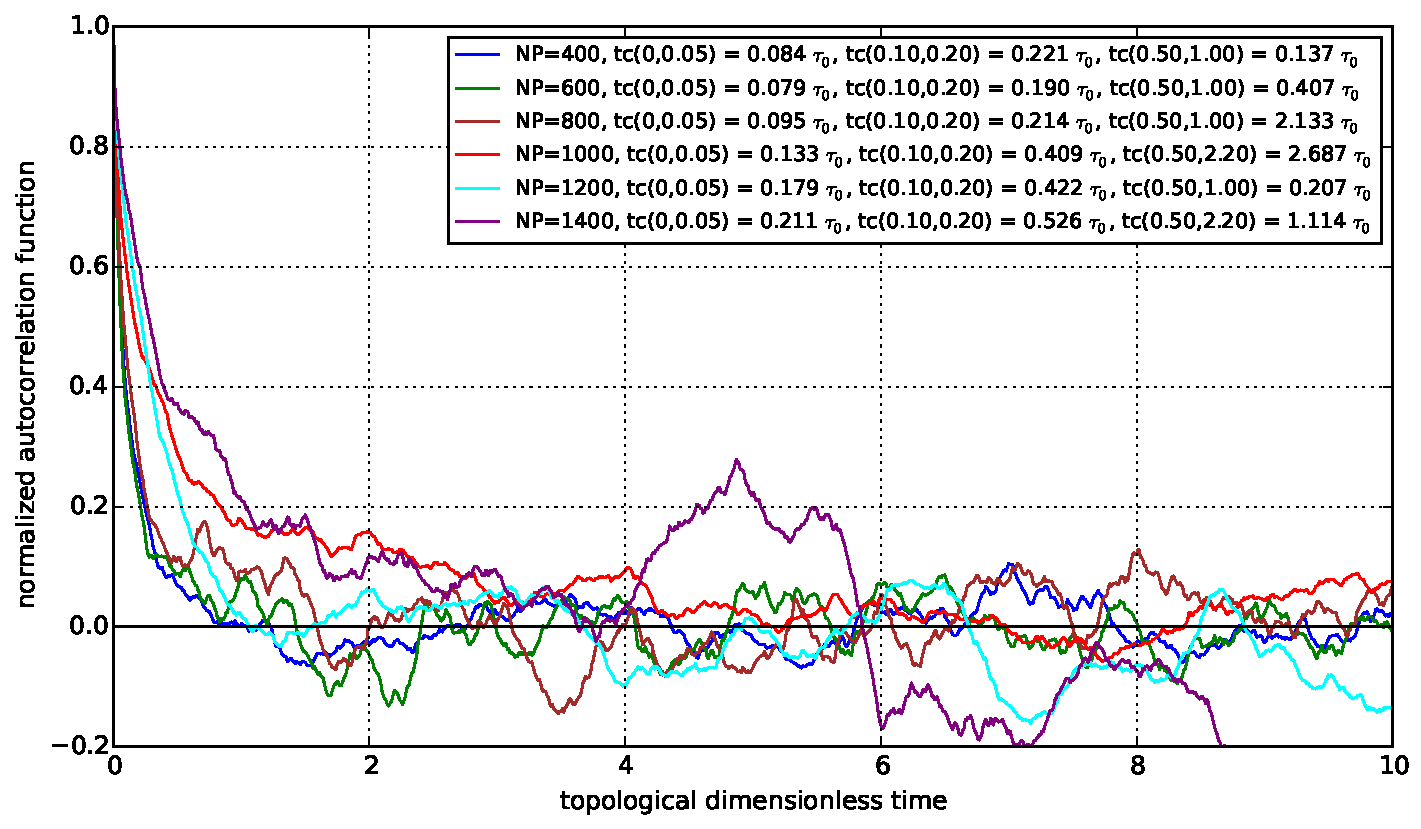
\includegraphics[width=\textwidth]{../check_ACF_NP.pdf}
  \end{figure}
\end{frame}

\begin{frame}
  \frametitle<presentation>{ACF for Shear Stress, biased statistics}
  \begin{figure}
    \centering
    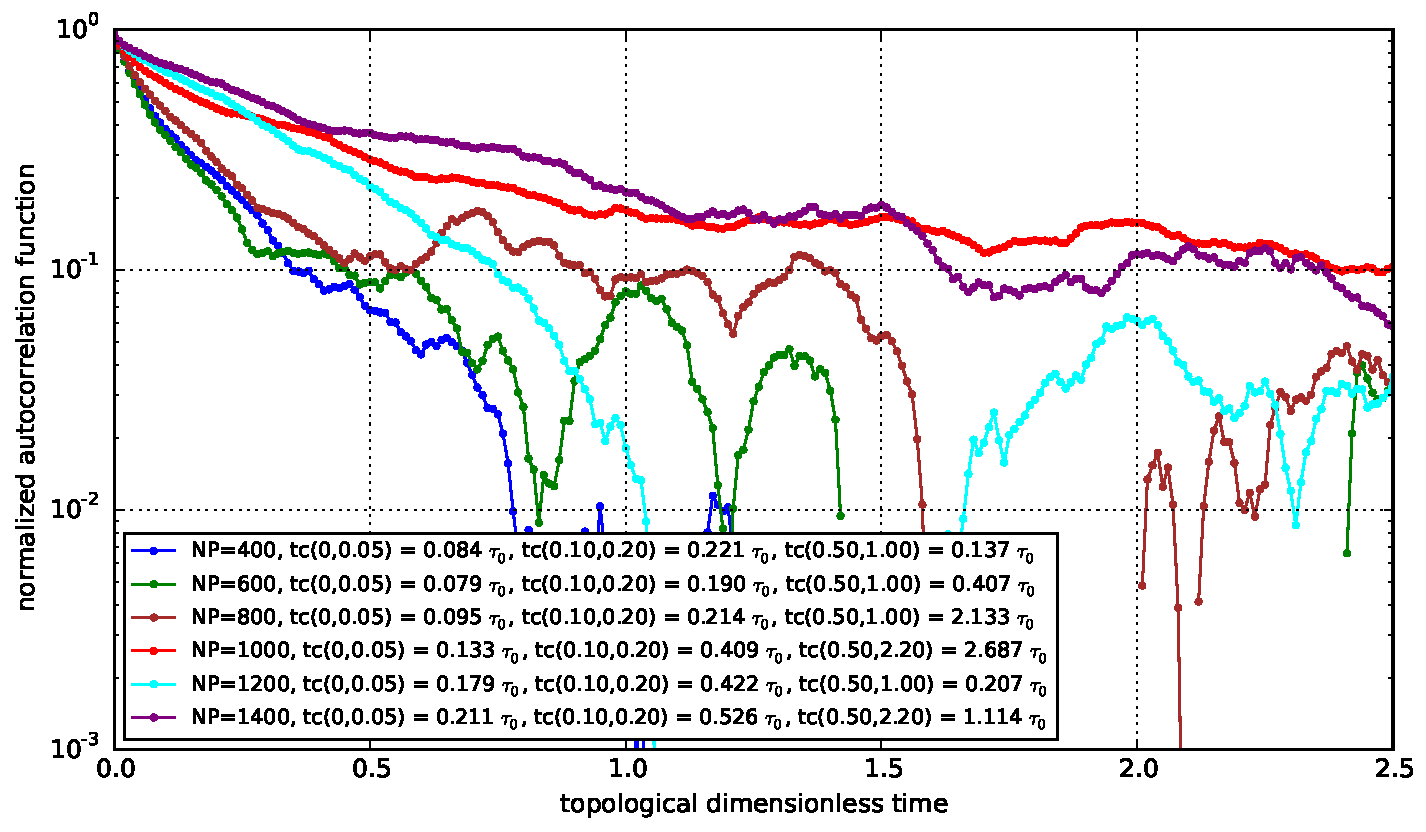
\includegraphics[width=\textwidth]{../check_ACF_NP_semilogy.pdf}
  \end{figure}
\end{frame}

\begin{frame}
  \frametitle<presentation>{ACF for Shear Stress, biased statistics}
  \begin{figure}
    \centering
    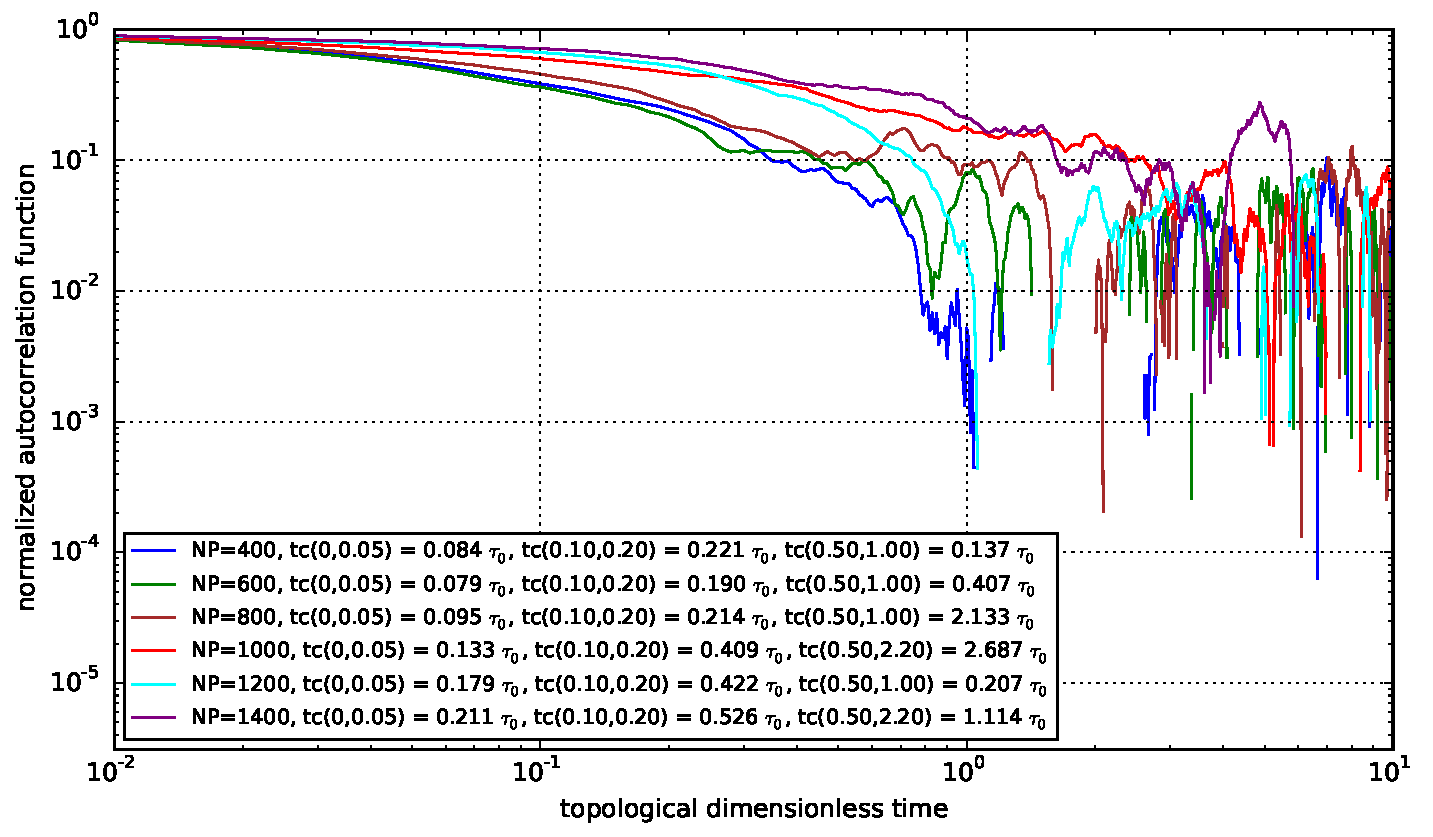
\includegraphics[width=\textwidth]{../check_ACF_NP_loglog.pdf}
  \end{figure}
\end{frame}


% \begin{frame}
%   \frametitle<presentation>{Average detachment frequency and dissociation time}
%   \begin{figure}
%     \centering
%     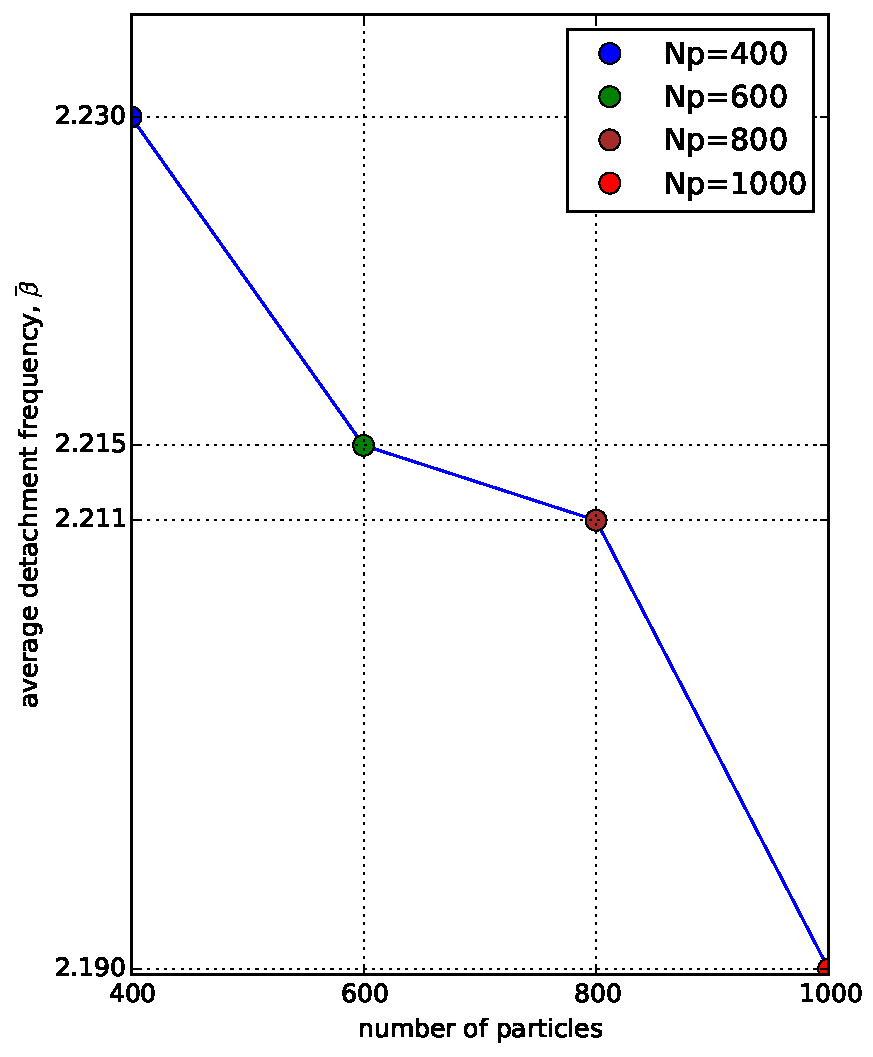
\includegraphics[width=0.45\textwidth]{../check_beta.pdf}
%     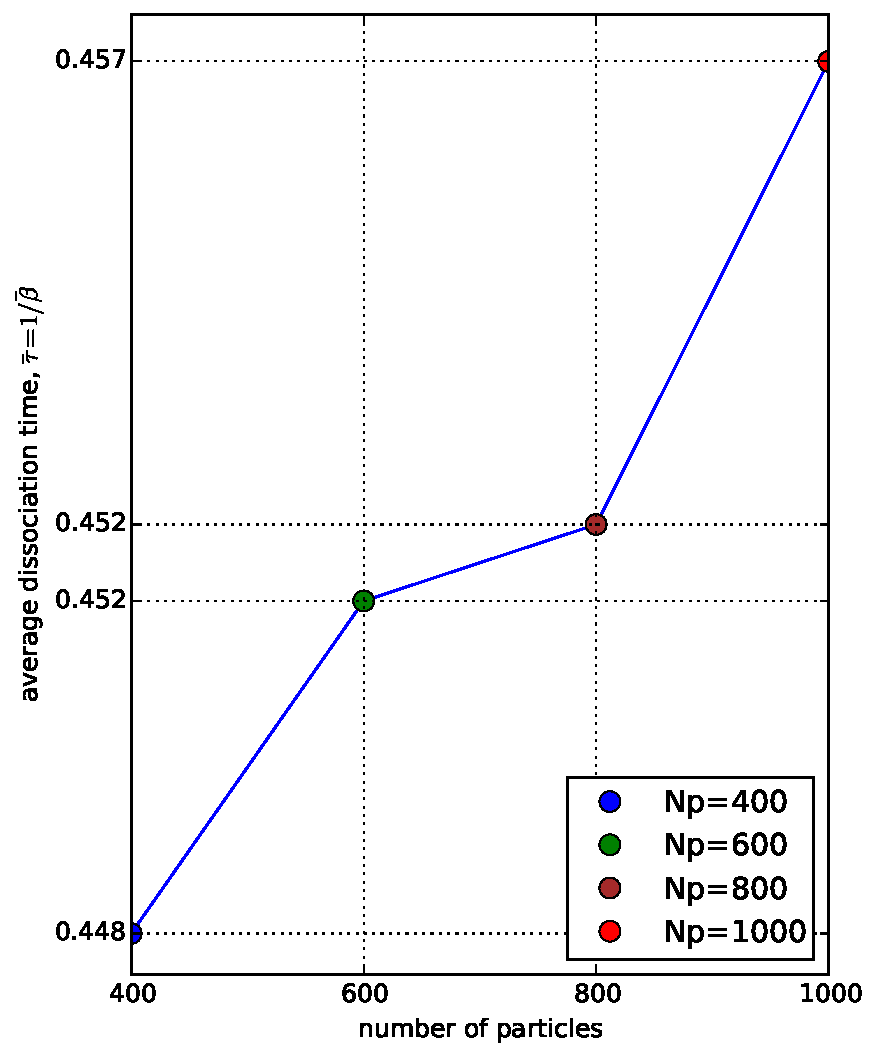
\includegraphics[width=0.45\textwidth]{../check_tau.pdf}
%   \end{figure}
% \end{frame}

\begin{frame}
  \frametitle<presentation>{Correlation time}
  \begin{figure}
    \centering
    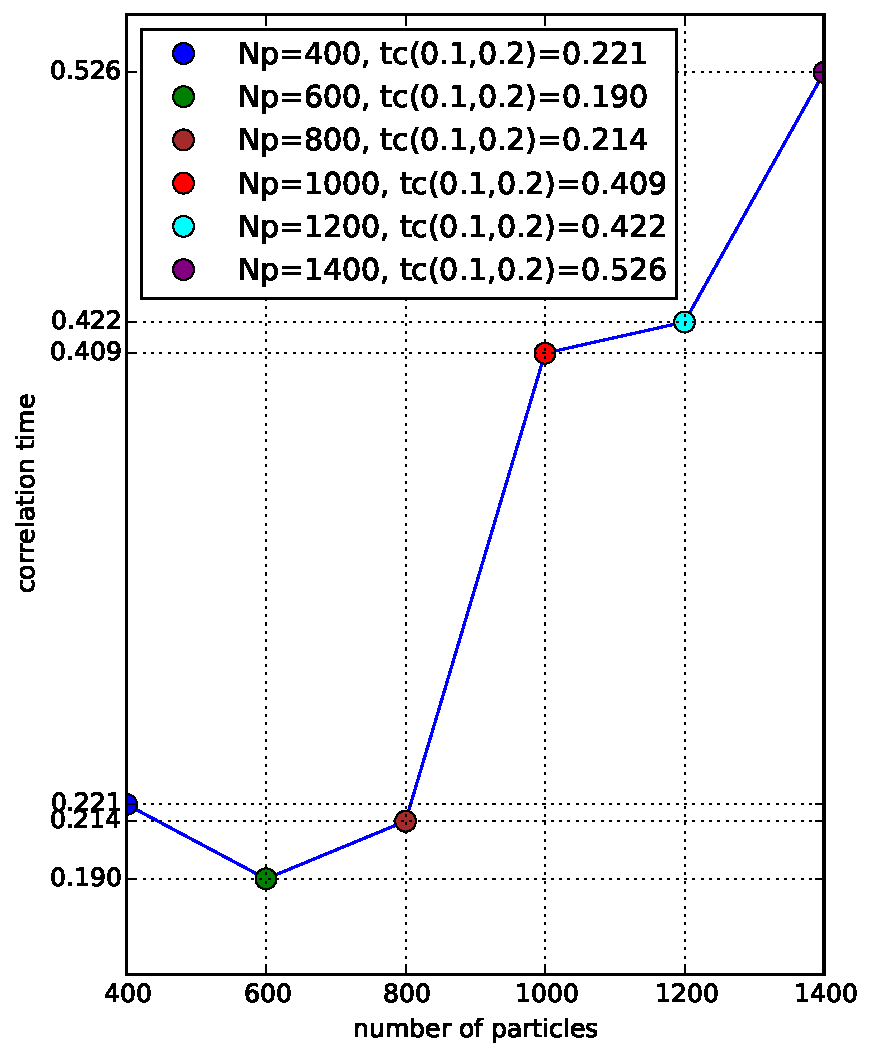
\includegraphics[width=0.45\textwidth]{../check_tc1.pdf}
    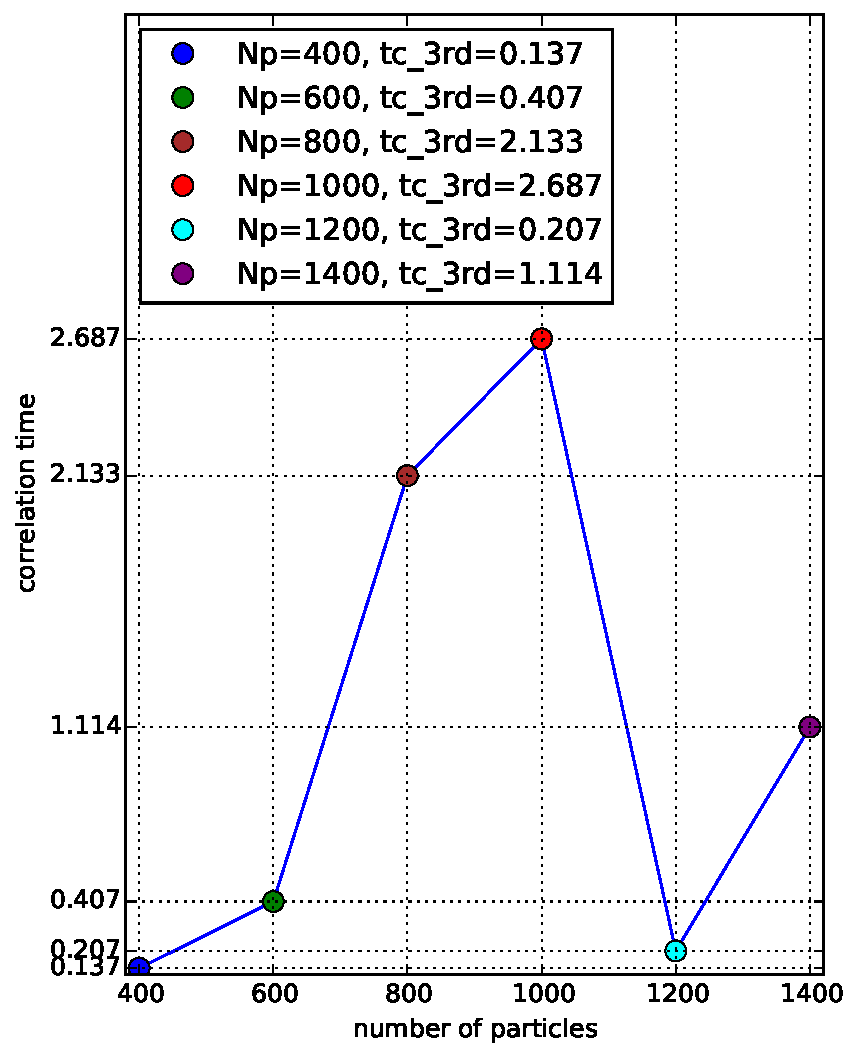
\includegraphics[width=0.45\textwidth]{../check_tc2.pdf}
  \end{figure}
\end{frame}

% \begin{frame}
%   \frametitle<presentation>{Correlation time and average detachment frequency}
%   \begin{figure}
%     \centering
%     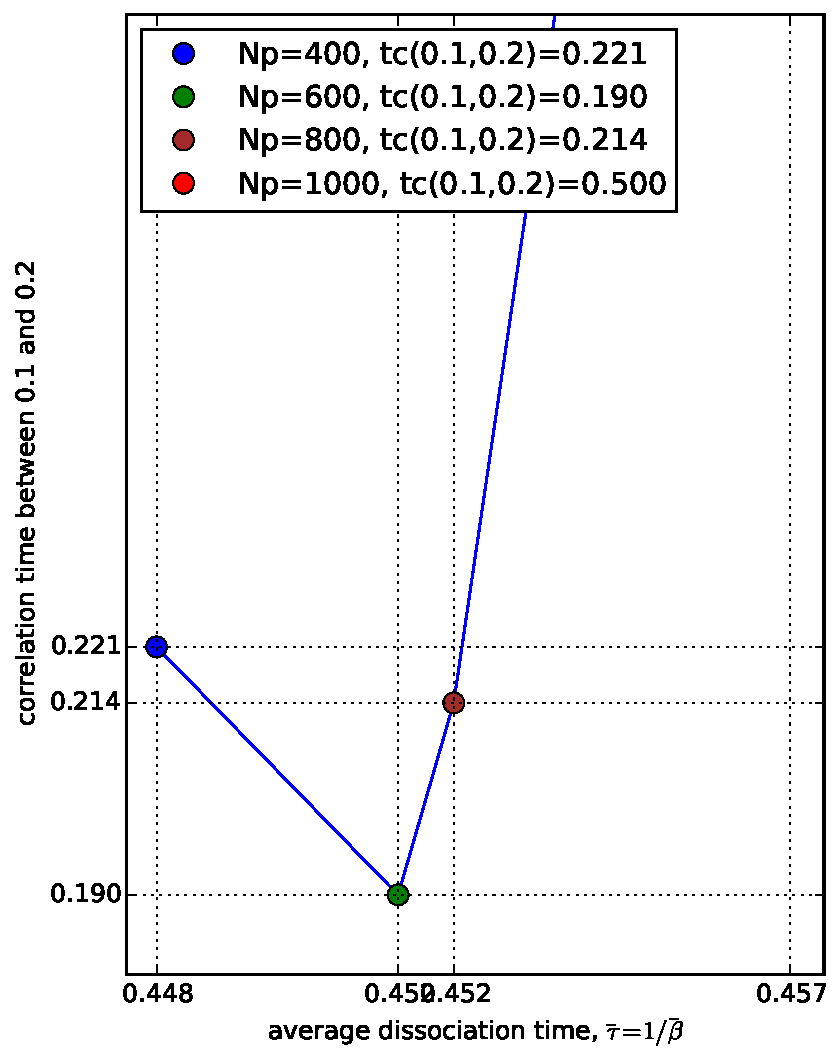
\includegraphics[width=0.45\textwidth]{../check_tc_01_02_beta.pdf}
%     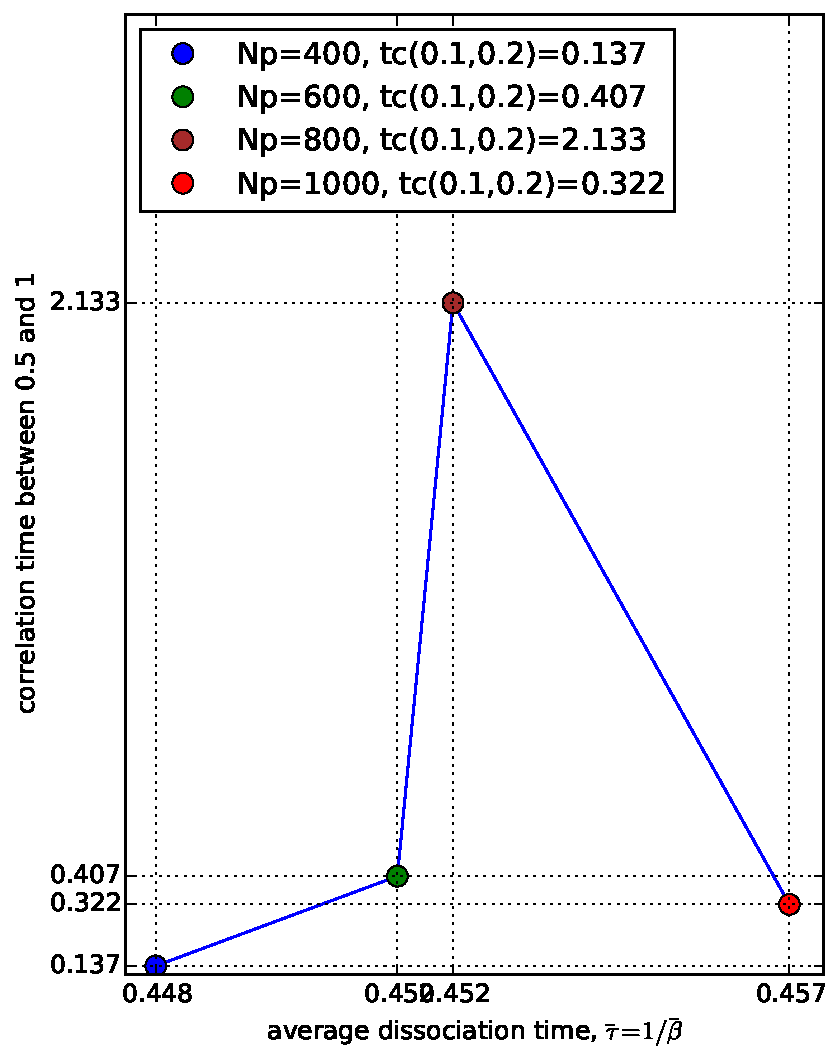
\includegraphics[width=0.45\textwidth]{../check_tc_05_1_beta.pdf}
%   \end{figure}
% \end{frame}


\begin{frame}
  \frametitle<presentation>{Test Condition}
  \begin{block}{Current definition for time scales}
  \begin{align}
    \tau_0 &= \beta_0^{-1}\quad\textrm{dissociation time}\\
    \tau_B &= \frac{R_0^2\zeta}{k_BT}\frac{1}{C},\quad\textrm{Brownian time}.
  \end{align}
  As a default, the rational time scale, $R_t = \tau_0/\tau_B$, is set by 100.
  \end{block}
  \begin{itemize}
  \item time step for Brownian motion: $10^{-4}\tau_0$ (=$10^{-2}\tau_B$)
  \item time step for topology: $10^{-3}\tau_0$ (=$10^{-1}\tau_B$)
  \item data output frequency: $10^{-2}\tau_0$ (=$\tau_B$)
  \end{itemize}
\end{frame}


\end{document}